\documentclass[11pt,wide]{mwart}
\usepackage[utf8]{inputenc} 
\usepackage[OT4,plmath]{polski}
\usepackage{graphicx}
\usepackage{caption}
\usepackage{subcaption}
\usepackage{epstopdf}
\usepackage{alltt}
\usepackage[section]{placeins}
\usepackage{graphicx}

\usepackage{amsmath,amssymb,amsfonts,amsthm,mathtools}


\usepackage{bbm}
\usepackage{hyperref}
\usepackage{url}

\usepackage{comment}

\date{Wrocław, \today}
\title{\LARGE\textbf{Pracownia z analizy numerycznej}
  \\Sprawozdanie do zadania \textbf{P1.16.}}

\author{Maciej Buszka}

\newtheorem{tw}{Twierdzenie}
\newtheorem{alg}{Algorytm}

\begin{document} 
\maketitle
\thispagestyle{empty}
\tableofcontents

\section{Wstęp}

Problem rozwiązania układu równań nieliniowych jest często napotykany w fizyce, matematyce i informatyce. Także w tych dziedzinach wiele innych problemów można  zredukować do problemu znalezienia pierwiastków układu równań nieliniowych. W tym sprawozdaniu opiszę metodę Newtona, czyli iteracyjny algorytm znajdujący pierwiastek funkcji $ F : \mathbb{R}^n \rightarrow \mathbb{R}^n $, czyli rozwiązanie równania $ F(x) = 0 $. Na podstawie różnych testów numerycznych zbadam zbieżność oraz zachowanie tej metody dla małych i dużych układów równań liniowych.

\section{Metoda Newtona}

\subsection{Intuicja i opis}

Dla funkcji jednej zmiennej $ f(x) = y $ metoda Newtona opiera się na założeniu że w okolicach punktu $ x_n $ możemy przybliżyć funkcję $ f $ funkcją liniową $ l(x) = f'(x_n)(x - x_n) + f(x_n) $. Można łatwo przekształcić ten wzór tak aby znaleźć miejsce zerowe tej funkcji liniowej.

\begin{equation} \label{eq:newtonsimple}
		x_{n+1} = x_n - \frac{f(x_n)}{f'(x_n)}
\end{equation}

Otrzymaną zależność możemy zinterpretować następująco: jeżeli $ x_n $ jest wystarczająco blisko miejsca zerowego $ \alpha $ funkcji $ f $, to chcielibyśmy znaleźć taką poprawkę $ h $ aby $ f(x_n + h) = f(\alpha) = 0 $. Korzystając ze wzoru Taylora $ f(x_n + h) = f(x_n) + f'(x_n)h + \dots $ zakładając, że $ x_n $ jest blisko $ \alpha $ otrzymujemy równanie $ h = -\frac{f(x_n)}{f'(x_n)} $. Zatem z równania \eqref{eq:newtonsimple} $ f(x_{n+1}) \approx 0 $ co pokazuje, że taka zależność może dać ciąg zbieżny do $ \alpha $.\\
 
Analogiczne rozumowanie chcielibyśmy teraz przeprowadzić dla funkcji $ F : \mathbb{R}^n \to \mathbb{R}^n $. Można ją zapisać w postaci wektora funkcji:

$$ 
F(x) = F(x_1, x_2, \ldots, x_n) = 
\left(\begin{matrix}
	f_1(x_1, x_2, \ldots, x_n) \\ 
	f_2(x_1, x_2, \ldots, x_n) \\ 
	\vdots\\ 
	f_n(x_1, x_2, \ldots, x_n)
\end{matrix}\right)
$$

\noindent Jeżeli funkcja $ F $ jest różniczkowalna w punkcie $ x $, to macierz jej pochodnych cząstkowych nazywana Jakobianem jest macierzą przekształcenia liniowego, które jest najlepszym przybliżeniem $ F $

$$ J = 
\begin{pmatrix}
\frac{\partial f_1}{\partial x_1} & \frac{\partial f_1}{\partial x_2} &  \ldots & \frac{\partial f_1}{\partial x_n} \\ 

 \vdots & & & \vdots  \\ 
\frac{\partial f_n}{\partial x_1} & \frac{\partial f_n}{\partial x_2} &  \ldots & \frac{\partial f_n}{\partial x_n} \\ 
\end{pmatrix}
$$

\noindent Korzystając ze wzoru Taylora dla funkcji $ F $ w punkcie $ x^{(n)} $ chcielibyśmy aby $ h$ było taką poprawką, że $ F(x^{(n)} + h) = 0 $

$$
 	0 = F(x^{(n)} + h) \approx F(x^{(n)}) + J(x^{(n)})h
$$

\noindent Stąd

\begin{equation} \label{eq:newtonH}
	J(x^{(n)})h = -F(x^{(n)})
\end{equation}

\noindent Jeśli J jest odwracalna, to możemy przekształcić równanie \eqref{eq:newtonH} do postaci
$$ 
	h = -J^{-1}(x^{(n)})F(x^{(n)}) 
$$

\noindent I wykorzystać tę zależność do znalezienia następnego przybliżenia miejsca zerowego funkcji $ F $

\begin{equation} \label{eq:newtonrec}
	x^{(n + 1)} = x^{(n)} + h
\end{equation}
\begin{equation*}
	x^{(n + 1)} = x^{(n)} - J^{-1}(x^{(n)})F(x^{(n)})
\end{equation*}

\noindent Niestety, aby bezpośrednio wykorzystać powyższe równanie musielibyśmy w każdym kroku  obliczać odwrotność macierzy $ J(x^{(n)}) $, co jest kosztowne ($ O(\frac{4}{3}n^3) $)\footnote{\cite{kincaid} Kincaid str.~169.}. Zamiast tego lepiej bezpośrednio rozwiązać równanie \eqref{eq:newtonH} i otrzymane $ h $ podstawić do wzoru \eqref{eq:newtonrec}

\subsection{Analiza teorytyczna}

Zbieżność metody Newtona dogłębnie analizują J.~C.~Ortega oraz W.~C.~Rheinboldt w \cite{ortega}. Przytoczę tutaj najważniejsze z twierdzeń.

\begin{tw}
Załóżmy, że $ F : D \subset \mathbb{R}^n \rightarrow \mathbb{R}^n $ jest różniczkowalna w otwartym otoczeniu $ S_0 \subset D $ punktu $ x^* $ takiego, że $ F(x^*) = 0 $, $ J = F' $ jest ciągła w $ x^* $ oraz macierz $ J(x^*) $ jest nieosobliwa, to metoda Newtona jest zbieżna nadliniowo dla $ x^{(0)} \in S_0 $. Jeśli ponadto pochodna $ F' $ jest ciągła na $ S_0 $ oraz druga pochodna $ F'' $ istnieje w $ x^* $ oraz 
\begin{align}
	\forall h \in \mathbb{R}^n, h \neq 0 \quad F''(x^*)hh \neq 0
\end{align}
to metoda Newtona jest zbieżna kwadratowo
\end{tw}

\begin{proof}
	Udowodnione w \cite{ortega} str 312-313
\end{proof}

\subsection{Implementacja}

Metodę Newtona bardzo łatwo zaimplementować, o ile założymy, że Jakobian funkcji jest nam dany. W poniższym algorytmie zakładamy, że przekazane są $ F $ - funkcja, $ J $ - pochodna tej funkcji, $ x $ - przybliżenie początkowe oraz kryteria zatrzymania: \texttt{eps} - tolerowany błąd względny przybliżenia oraz wartości funkcji i \texttt{imax} - maksymalna liczba iteracji. W algorytmie wykorzystuję funkcję biblioteczną \texttt{norm(x)}, która oblicza normę wektora $ x $. Definiuję także funkcję \texttt{solve(A, b)}, która rozwiązuje układ równań $ Ax = b $. Na potrzeby tego algorytmu została ona zaimplentowana metodą eliminacji Gaussa.

\begin{verbatim}
		Dane: F, J, x, eps = 1e-12, imax = 20
		Wynik : x
		
		i := 0
		ex := 1.0
		ef := 1.0
		Jx := J(x)
	    Fx := F(x)
	    
		while (ex > eps or ef > eps) and i < imax do
		  i  := i + 1
		  h  := solve(Jx, Fx)
		  ex := norm(h) / norm(x)
		  x  := x - h
		  Jx := J(x)
		  Fx := F(x)
		  ef := norm(Fx)
		done			
\end{verbatim}

Algorytm został zaimplentowany w języku Julia w pliku \texttt{newton.jl}

\subsection{Koszt obliczeniowy iteracji}

W każdej iteracji głównej pętli metody Newtona musimy wykonać następujące kosztowne działania:

\begin{enumerate}
\item Obliczenie wartości funkcji $ F(x) $
\item Obliczenie wartości jakobianu $ J(x) $
\item Obliczenie norm $ x $, $ F(x) $ i $ h $: \quad $ O(n) $
\item Rozwiązanie układu równań $ J(x)h = F(x)$: \quad  $ O(\frac{1}{3}n^3 + \frac{3}{2}n^2) $
\end{enumerate}

Koszt dwóch pierwszych nie jest zależny od implementacji metody Newtona, koszt trzeciej jest liniowy względem wielkości wektora, natomiast koszt rozwiązania układu równań jest przeanalizowany w \S \ref{SS:gausscost}

\section{Metoda eliminacji Gaussa}

\subsection{Opis} \label{p:gaussopis}

Metoda eliminacji Gaussa jest najprostszym koncepcyjnie algorytmem rozwiązywania układu równań liniowych postaci $ Ax = b $.
Składa się on z dwóch faz: eliminacji i podstawiania.

Rozważmy następujący układ:

$$
\left(\begin{matrix}
a_{11} & a_{12} & \ldots & a_{1n} \\
a_{21} & a_{22} & \ldots & a_{2n} \\
\vdots & \vdots & 		 & \vdots \\
a_{i1} & a_{i2} & \ldots & a_{in} \\
\vdots & \vdots & 		 & \vdots \\
a_{n1} & a_{n2} & \ldots & a_{nn}
\end{matrix}\right)
\left(\begin{matrix}
x_1 \\ x_2 \\ \vdots \\ x_i \\ \vdots \\ x_n
\end{matrix}\right) = 
\left(\begin{matrix}
b_1 \\ b_2 \\ \vdots \\ b_i \\ \vdots \\ b_n
\end{matrix}\right)
$$

\noindent W fazie eliminacji chcemy sprowadzić go do postaci górnotrójkątnej tj.

$$
\left(\begin{matrix}
a_{11} & a_{12} &  & \ldots  & & a_{1n} \\
0 & a_{22} &  & \ldots  & & a_{2n} \\
\vdots & \vdots & \ddots &		 & & \vdots \\
0 & 0 & \ldots & a_{ii}  & \ldots & a_{in} \\
\vdots & \vdots &  &		 & \ddots & \vdots \\
0 & 0 &  & \ldots  & 0 & a_{nn}
\end{matrix}\right)
\left(\begin{matrix}
x_1 \\ x_2 \\ \vdots \\ x_i \\ \vdots \\ x_n
\end{matrix}\right) = 
\left(\begin{matrix}
b_1 \\ b_2 \\ \vdots \\ b_i \\ \vdots \\ b_n
\end{matrix}\right)
$$

Możemy to osiągnąć odejmując odpowiednią wielokrotność pierwszego wiersza od pozostałych, a następnie powtarzając ten krok dla macierzy z obciętym pierwszym wierszem i kolumną. Tak więc w $ k $-tym powtórzeniu procedury musimy wykonać następujące podstawienia:

\begin{equation}
\begin{cases}
	\alpha_k \leftarrow \frac{a_{ik}}{a_{kk}} \\
	a_{ij} \leftarrow a_{ij} - \alpha_k a_{kj} \\
	b_{i} \leftarrow b_{i} - \alpha_k b_{i}
\end{cases} \text{ dla }(k \leq j \leq n), (k + 1 \leq i \leq n)
\end{equation}

Współczynnik $ \alpha_k $ nazywamy mnożnikiem, natomiast wyraz $ a_{kk} $ elementem głównym, względem którego redukujemy układ. Gdy już otrzymamy macierz w postaci górnotrójkątnej, aby otrzymać wynik wystarczy wykonać następujące podstawienia:
$$ 
\begin{cases}
	x_n \leftarrow \frac{b_n}{a_{nn}} \\
	x_k \leftarrow \frac{b_k - \sum_{j = k+1}^{n} a_{kj}x_{j}}{a_{kk}} \quad \text{ dla } k = (n-1, \ldots ,  1)
\end{cases}
$$

\subsection{Znaczenie elementów głównych}

Podczas implementacji metody eliminacji Gaussa największym problemem jest wybór wiersza, względem którego będziemy wykonywać eliminację. Po pierwsze, nie może on mieć zerowego elementu głównego. Po drugie, jeżeli będzie on bardzo mały względem innych elementów w tej kolumie macierzy, natrafimy na błędy wynikające z dodawania i odejmowania bardzo dużych liczb. Rozważmy dla przykładu układ równań:

\begin{align} \label{eq:gaussfail}
\left(\begin{matrix}
\epsilon & 1	\\
       1 & 1
\end{matrix}\right)
\left(\begin{matrix}
x_1 \\ x_2
\end{matrix}\right) = 
\left(\begin{matrix}
1 \\ 2
\end{matrix}\right)
\end{align}

\noindent W pierwszym (i jedynym) kroku eliminacji przekształcony zostanie on do postaci

\begin{align*}
\left(\begin{matrix}
\epsilon & 1	\\
 0 & 1 - \epsilon^{-1}
\end{matrix}\right)
\left(\begin{matrix}
x_1 \\ x_2
\end{matrix}\right) = 
\left(\begin{matrix}
1 \\ 2 - \epsilon^{-1}
\end{matrix}\right)
\end{align*}

\noindent Ma on rozwiązania 

$$ 
x_2 = \frac{2 - \epsilon^{-1}}{1 - \epsilon^{-1}} \approx 1 \quad x_1 = \frac{(1 - x_2)}{\epsilon} \approx 1
$$

\noindent Jednak przy obliczaniu tych wartości w komputerze, dla odpowiednio małego $ \epsilon $,  $ fl(2 - \epsilon^{-1}) = fl(1 - \epsilon^{-1}) = fl(\epsilon^{-1}) $ co daje nam $ x_2 = 1 $ i $ x_1 = 0 $, co jest absurdalnym wynikiem.

Gdyby poprzedni układ zapisać w postaci

\begin{align*}
\left(\begin{matrix}
       1 & 1 \\
\epsilon & 1
\end{matrix}\right)
\left(\begin{matrix}
x_1 \\ x_2
\end{matrix}\right) = 
\left(\begin{matrix}
2 \\ 1
\end{matrix}\right)
\end{align*}

\noindent otrzymalibyśmy poprawny wynik, co jest pokazane w \cite{kincaid} str.~162-163. Widzimy zatem, że konieczne jest odpowiednie wybranie wiersza, względem którego wykonamy redukcję.

\subsection{Implementacja}

Wykorzystamy algorytm eliminacji Gaussa ze skalowanym wyborem wierszy głównych opisany w \cite{kincaid} str.~165-166. Radzi on sobie z zerowymi oraz znacząco różnymi elementami głównymi macierzy permutując na bieżąco kolejność wierszy. Na początku tworzymy wektor skal $ s_i = \max_{1 \leq k \leq n}a_{ik} $, po czym w \texttt{k}-tym kroku wybieramy wiersz w którym iloraz $ \frac{a_{kj}}{s_j} (j = k, k+1, \ldots,n)$ jest najmniejszy. Poza tą modyfikacją algorytm jest jak w \S\ref{p:gaussopis}. Jego implementacja w języku Julia znajduje się w pliku \texttt{gauss.jl}

\subsection{Koszt} \label{SS:gausscost}

Rozważając koszt algorytmu zliczamy tzw. długie operacje, czyli pary mnożenie/dzielenie i dodawanie/odejmowanie. W pierwszym kroku algorytmu należy wybrać wiersz, względem którego wykonana zostanie eliminacja, co zajmuje $ n $ dzieleń, po czym dla pozostałych $ n - 1 $ wierszy obliczamy mnożnik ($ 1 $ dzielenie) i odejmujemy od niego wielokrotność wiersza pierwszego ($ n-1 $ mnożeń). Razem z wybraniem wiersza pierwszego zajmuje to $ n^2 $ operacji. W kolejnym kroku rozkładu wykonamy takie same operacje dla układu rozmiaru $ n - 1 $. Zatem koszt całego rozkładu to

\begin{equation*}
	n^2 + (n-1)^2 + \ldots + 3^2 + 2^2 = \frac{1}{3}n^3 + \frac{1}{2}n^2 + \frac{1}{6}n - 1 \approx \frac{1}{3}n^3 + \frac{1}{2}n^2
\end{equation*}

\noindent W trakcie podstawiania najpierw obliczamy wsp. $ b_i $ wykonując $ n-1, n-2, \ldots, 1 $, czyli łącznie $ \frac{n(n-1)}{2} $ mnożeń, a podstawiając wykonujemy $ 1, 2, \ldots, n-1, n $, czyli $ \frac{n(n+1)}{2} $ długich działań co łącznie daje koszt $ n^2 $ dla fazy podstawiania. Prowadzi to do następującego twierdzenia:

\begin{tw} 
Jeśli eliminację Gaussa wykonano ze skalowanym wyborem elementów głównych, to rozwiązanie układu $ Ax = b $ wymaga około $ \frac{1}{3}n^3 + \frac{3}{2}n^2 $ długich działań.\footnote{\cite{kincaid} Kincaid str.~168-169.}
\end{tw} 

\section{Wyniki eksperymentów}

\subsection{Znaczenie elementu głównego w eliminacji Gaussa}

Porównam tutaj zachowanie naiwnej implementacji eliminacji Gaussa i algorytmu ze skalowanym elementem głównym w arytmetyce podwójnej precyzji (typ danych \texttt{Float64}).

\begin{center}
\begin{table}[!htb]
\caption{Porównanie implementacji eliminacji Gaussa dla układu \eqref{eq:gaussfail}}
    \begin{subtable}{.5\linewidth}
      \centering
        \caption{naiwna}
\begin{tabular}{| c | c | c |} \hline
$ \epsilon $ & $x_1$ & $x_2$ \\ \hline
1.0e-01 & 1.1111111e+00 & 8.8888889e-01 \\ 
1.0e-02 & 1.0101010e+00 & 9.8989899e-01 \\
\vdots & \vdots & \vdots \\
1.0e-14 & 9.9920072e-01 & 1.0000000e+00 \\ 
1.0e-15 & 9.9920072e-01 & 1.0000000e+00 \\ 
1.0e-16 & \textbf{0.0000000e+00} & 1.0000000e+00 \\ 
1.0e-17 & \textbf{0.0000000e+00} & 1.0000000e+00 \\
\vdots & \vdots & \vdots \\ \hline
\end{tabular}
\end{subtable}%
\begin{subtable}{.5\linewidth}
\centering
\caption{ze skalowanym wyborem elementu głównego}
\begin{tabular}{| c | c | c |} \hline
$ \epsilon $ & $x_1$ & $x_2$ \\ \hline
1.0e-01 & 1.1111111e+00 & 8.8888889e-01 \\ 
1.0e-02 & 1.0101010e+00 & 9.8989899e-01 \\ 
\vdots & \vdots & \vdots \\
1.0e-14 & 1.0000000e+00 & 1.0000000e+00 \\ 
1.0e-15 & 1.0000000e+00 & 1.0000000e+00 \\ 
1.0e-16 & \textbf{1.0000000e+00} & 1.0000000e+00 \\ 
1.0e-17 & \textbf{1.0000000e+00} & 1.0000000e+00 \\
\vdots & \vdots & \vdots \\ \hline
\end{tabular}
\end{subtable}
\label{tab:gauss}
\end{table} 
\end{center}

Jak widać w tabeli \ref{tab:gauss} dla $ \epsilon \leq 10^{-16} $ naiwna implementacja  metody eliminacji Gaussa daje złe rozwiązanie ($ x_1 = 0 $), natomiast zaimplementowanie skalowanego wyboru elementu głównego daje poprawny wynik ($ x_1 = 1 $).

\subsection{Małe układy równań}

Pokazane są tutaj przebiegi metody Newtona dla dwóch funkcji $ F_1 $ i $ F_5 $, a także porównanie tempa zbieżności wszystkich funkcji testowych, których wzory można zobaczyć w zeszycie interaktywnym \texttt{program.ipynb} za pomocą programu \texttt{jupyter}.

\begin{align*}
F_1(x) = 
\left(\begin{matrix}
	(x_1)^2 + (x_2)^2 - 25 \\
	(x_1)^2 - x_2 - 2
\end{matrix}\right) && F_5(x) =
\left(\begin{matrix}
(x_1)^3 + 7(x_2)^2 - 7 \\
(x_1)^2 + (x_2)^2 - 1
\end{matrix}\right)
\end{align*}

\begin{center}
\begin{table}[!htb]
\caption{Porównanie zbieżności metody Newtona}
    \begin{subtable}{.5\linewidth}
      \centering
      \caption{Obserwowana zbieżność kwadratowa dla funkcji $ F_1 $}
\begin{tabular}{| c | c | c |} \hline
Iteracja & $\|F(x)\|$ & $\epsilon$ \\ \hline
1 & 7.215002e+01 & 5.884301e+00 \\ 
2 & 1.347658e+01 & 3.675183e-01 \\ 
3 & 1.263553e+00 & 1.725992e-01 \\ 
4 & 2.271418e-02 & 2.592261e-02 \\ 
5 & 1.219716e-05 & 5.889474e-04 \\ 
6 & 4.119923e-12 & 3.413509e-07 \\ 
7 & 8.881784e-16 & 1.158651e-13 \\  \hline
\end{tabular}
      \caption*{Przybliżenie początkowe $ x_0 = (1, 1)^T $}
\end{subtable}%
\begin{subtable}{.5\linewidth}
\centering
\caption{Obserwowana zbieżność liniowa dla funkcji $ F_5 $}
\begin{tabular}{ |c | c | c| } \hline
Iteracja & $\|F(x)\|$ & $\epsilon$ \\ \hline
1 & 2.154066e+01 & 1.264911e+00 \\ 
2 & 1.532314e+01 & 8.820599e-01 \\ 
3 & 3.678398e+00 & 4.438798e-01 \\ 
\vdots & \vdots & \vdots \\
15 & 3.998377e-08 & 1.999594e-04 \\ 
16 & 9.994226e-09 & 9.997112e-05 \\ 
17 & 2.498342e-09 & 4.998342e-05 \\ 
18 & 6.245589e-10 & 2.499117e-05 \\ 
19 & 1.561364e-10 & 1.249545e-05 \\ 
20 & 3.903389e-11 & 6.247696e-06 \\  \hline
\end{tabular}
\caption*{Przybliżenie początkowe $ x_0 = (1, 2)^T $}
\end{subtable}
\end{table}
\end{center}

Na poniższych wykresach jako wskaźnik dokładności przyjąłem wartość $ y = -\log_{10}\epsilon $ dla błędu względnego oraz $ y = -\log_{10}\|F(x)\| $ dla wartości funkcji.

\begin{figure}[h]
    \centering
    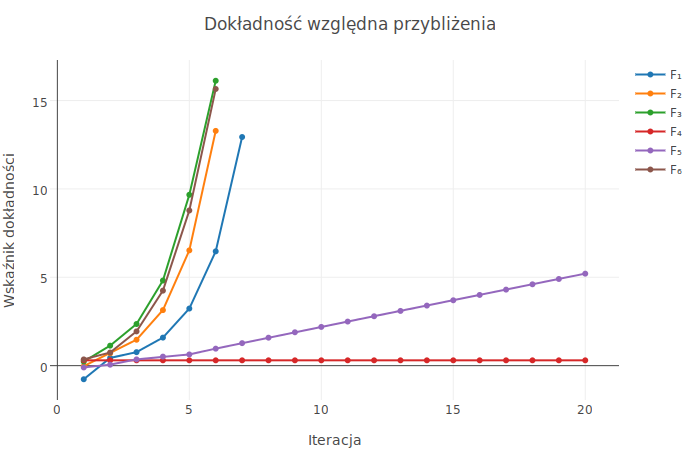
\includegraphics[width=0.8\textwidth]{rel_precision}
    \caption{Porównanie względnej dokładności przybliżenia dla różnych funkcji}
    \label{fig:relprecision}
\end{figure}

\begin{figure}[h]
    \centering
    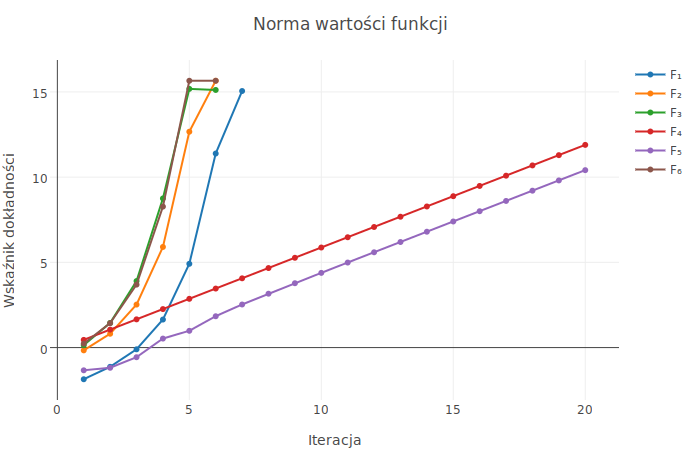
\includegraphics[width=0.8\textwidth]{norm}
    \caption{Porównanie wartości $ \| F(x) \| $ dla różnych funkcji}
    \label{fig:norm}
\end{figure}

\FloatBarrier
\subsection{Duże układy równań}

Tutaj porównam ilość iteracji metody Newtona potrzebną do znalezienia pierwiastka funkcji o $ n $ niewiadomych. Testy przeprowadzono dla czterech funkcji, dla każdej z nich jednym z miejsc zerowych jest wektor $ \bar{x} = (1, 1, \ldots, 1)^T $, natomiast przybliżenie początkowe to wektor $ x^{(0)} = (x_1, x_2, \ldots, x_n )$ o losowo wybranych współczynnikach $ x_i \in (1-\delta, 1+\delta) $. Zbadałem następujące funkcje

\begin{align}
	F(x) &= 
	\left(\begin{matrix}
		f_1(x) - f_1(\bar{x}) \\ 
		f_2(x) - f_2(\bar{x}) \\ 
		\vdots\\ 
		f_n(x) - f_n(\bar{x})
	\end{matrix}\right), && \text{dla} \quad f_i(x) = a_{ik}x_ix_k, \quad a_{ik} \in \{-10, -9, \ldots, 10 \} \label{eq:F}\\
	G(x) &=
	\left(\begin{matrix}
	g_1(x) - g_1(\bar{x}) \\ 
	g_2(x) - g_2(\bar{x}) \\ 
	\vdots\\ 
	g_n(x) - g_n(\bar{x})
\end{matrix}\right), && \text{dla} \quad g_i(x) = (x_i)^2\ + \sum_{k=1, k\neq i}^{n}\sin{x_i}cos{x_k} \label{eq:G}\\
	H(x) &= 
	\left(\begin{matrix}
	h_1(x) - h_1(\bar{x}) \\ 
	h_2(x) - h_2(\bar{x}) \\ 
	\vdots\\ 
	h_n(x) - h_n(\bar{x})
\end{matrix}\right), && \text{dla} \quad h_i(x) = 
		\begin{cases}  
			\sin{x_i}\sin{x_{i+1}}\cos{x_{i+2}}, & \text{ gdy } i \leq n-2 \\
			\sin{x_{n-1}}\sin{x_{n}}\cos{x_{1}}, & \text{ gdy } i = n - 1 \\
			\sin{x_n}\sin{x_{1}}\cos{x_{2}}, & \text{ gdy } i = n
		\end{cases} \label{eq:H} \\
	V(x) &=
	\left(\begin{matrix}
		v_1(x) - v_1(\bar{x}) \\ 
		v_2(x) - v_2(\bar{x}) \\ 
		\vdots\\ 
		v_n(x) - v_n(\bar{x})
	\end{matrix}\right), && \text{dla} \quad v_i(x) = x_1 + (i+1)x_2 + \ldots + (i+1)^{n-1}x_n \label{eq:V}
\end{align}

Dla każdej wartości $ n = 2, 3, \ldots, 20 $ i parametru $ \delta = 0.1, 0.2, 0.5, 1.0 $ przeprowadziłem 1000 prób, w których na nowo były losowane wektory początkowe oraz współczynniki $ a_{ik} $ dla funkcji $ F $. Wyniki wszystkich prób dla określonego $ n $ oraz $ \delta $ uśredniłem. Przyjąłem następujące kryteria zatrzymania iteracji:

\begin{itemize}
\item \texttt{maxiter =} $ 5n $ - maksymalna liczba iteracji (powstrzymuje program w przypadku rozbieżności).
\item $ \epsilon_s = 10^{-12} $ - zarówno tolerancja błędu względnego przybliżenia, jak i tolerancja normy wartości funkcji.
\end{itemize}

Obliczenia wykonane zostały dla typu danych \texttt{Float64}. Badając liczbę iteracji brałem pod uwagę jedynie przebiegi, w których metoda była zbieżna.

\begin{center}
\begin{table}[!htb]
\caption{Przykładowy przebieg metody Newtona dla układu rozmiaru $ n = 20 $ }
    \begin{subtable}{.5\linewidth}
      \centering
      \caption{Funkcja $ F $}
\begin{tabular}{ |c | c | c| } \hline
Iteracja & $\|F(x)\|$ & $\epsilon$ \\ \hline
0 & 7.113507e+01 & 4.435757e-01 \\ 
1 & 3.587656e+01 & 1.685290e-01 \\ 
2 & 3.579608e+00 & 2.631299e-02 \\ 
3 & 2.296047e-01 & 2.199988e-03 \\ 
4 & 7.829980e-04 & 1.532992e-05 \\ 
5 & 5.522215e-08 & 2.608613e-10 \\ 
6 & 3.436562e-14 & 2.343784e-16 \\  \hline
\end{tabular}
\end{subtable}%
\begin{subtable}{.5\linewidth}
\centering
\caption{Funkcja $ G $}
\begin{tabular}{| c | c | c |} \hline
Iteracja & $\|G(x)\|$ & $\epsilon$ \\ \hline
0 & 1.757268e+01 & 3.069187e-01 \\ 
1 & 1.323588e+01 & 1.108648e-01 \\ 
2 & 3.287417e+00 & 2.735830e-02 \\ 
3 & 2.506188e-01 & 1.954874e-03 \\ 
4 & 1.143128e-03 & 1.026775e-05 \\ 
5 & 3.456163e-08 & 2.875731e-10 \\ 
6 & 2.188678e-14 & 2.533492e-16 \\ \hline
\end{tabular}
\end{subtable}
\end{table}
\end{center}

\begin{figure}[h]
    \centering
    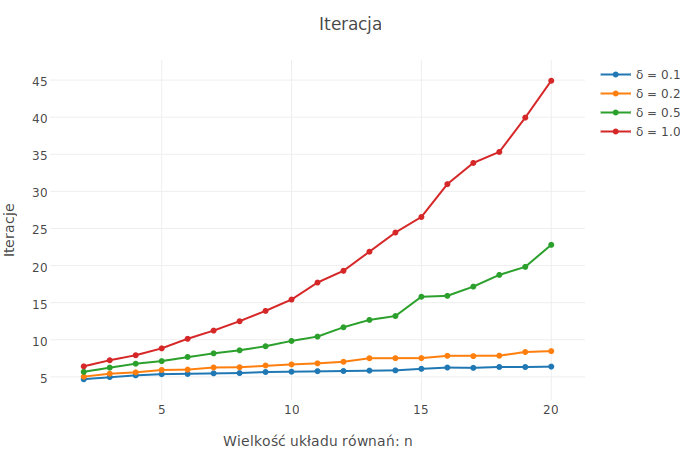
\includegraphics[width=0.9\textwidth]{avg_iterations_F}
    \caption{Średnia ilość iteracji potrzebna do zakończenia metody Newtona dla funkcji F \eqref{eq:F}}
    \label{fig:avgiterationsF}
\end{figure}

\begin{figure}[h]
    \centering
    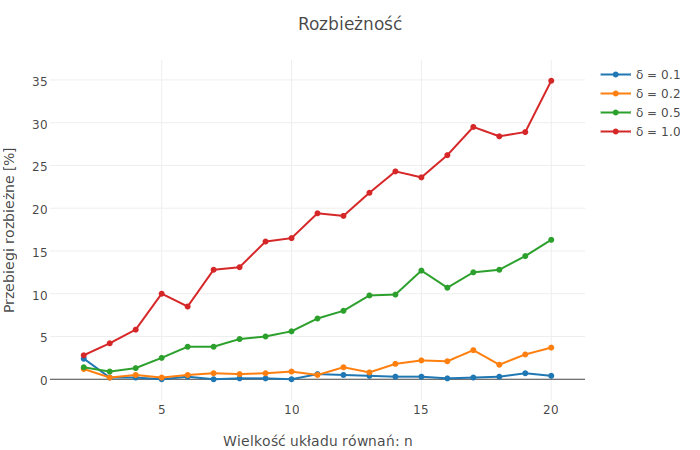
\includegraphics[width=0.9\textwidth]{avg_diversions_F}
    \caption{Procent uruchomień metody Newtona dla funkcji F \eqref{eq:F}, które nie zbiegły w limicie iteracji}
    \label{fig:avgdiversionsF}
\end{figure}

\begin{figure}[h]
    \centering
    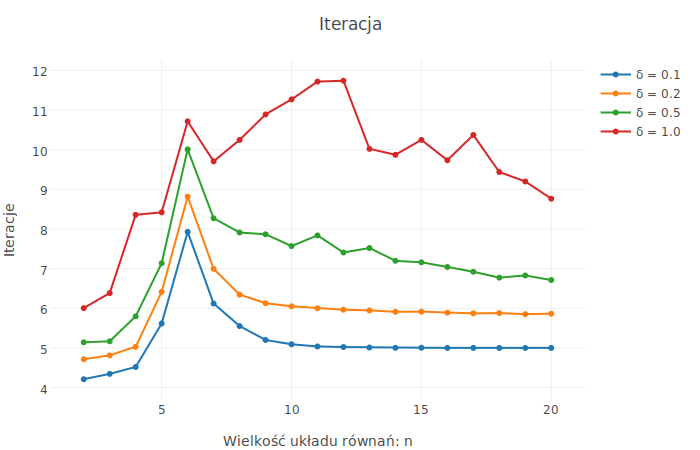
\includegraphics[width=0.9\textwidth]{avg_iterations_G}
    \caption{Średnia ilość iteracji potrzebna do zakończenia metody Newtona dla funkcji G \eqref{eq:G}}
    \label{fig:avgiterationsG}
\end{figure}

\begin{figure}[h]
    \centering
    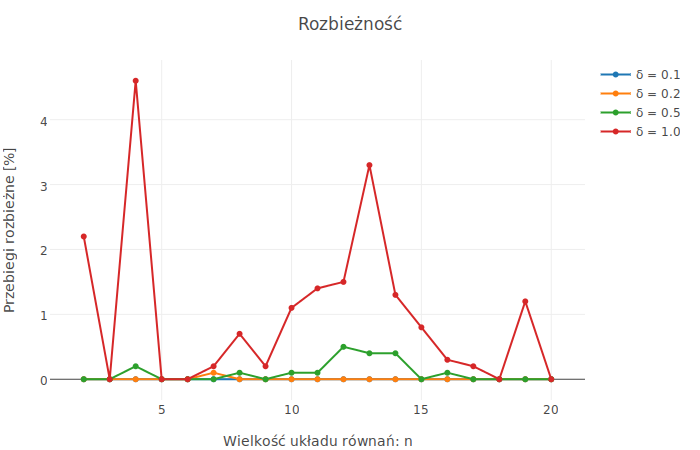
\includegraphics[width=0.9\textwidth]{avg_diversions_G}
    \caption{Procent uruchomień metody Newtona dla funkcji G \eqref{eq:G}, które nie zbiegły w limicie iteracji}
    \label{fig:avgdiversionsG}
\end{figure}

\begin{figure}[h]
    \centering
    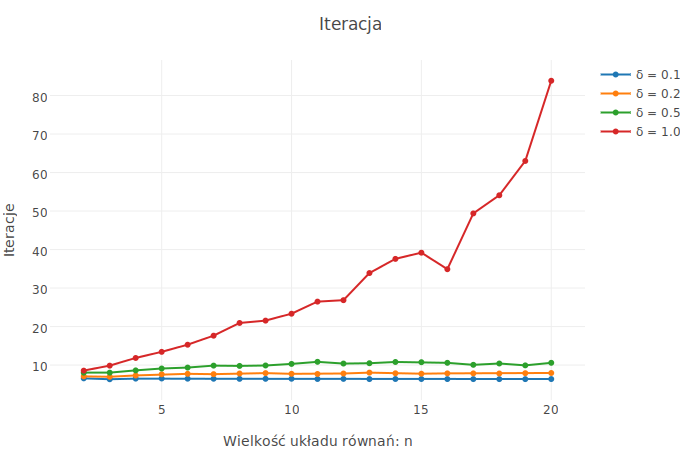
\includegraphics[width=0.9\textwidth]{avg_iterations_H}
    \caption{Średnia ilość iteracji potrzebna do zakończenia metody Newtona dla funkcji H \eqref{eq:H}}
    \label{fig:avgiterationsH}
\end{figure}

\begin{figure}[h]
    \centering
    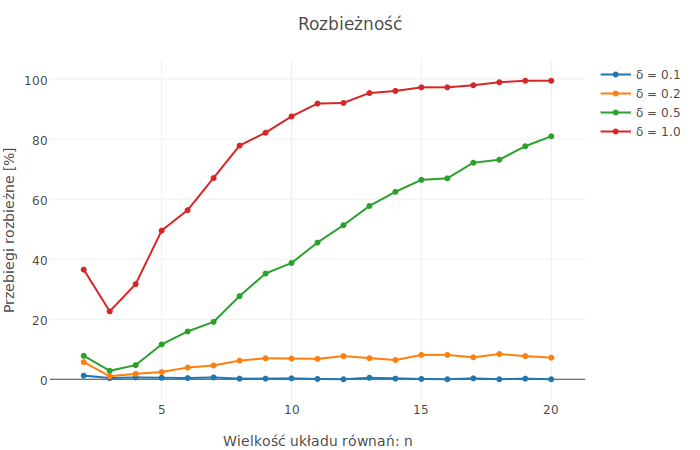
\includegraphics[width=0.9\textwidth]{avg_diversions_H}
    \caption{Procent uruchomień metody Newtona dla funkcji H \eqref{eq:H}, które nie zbiegły w limicie iteracji}
    \label{fig:avgdiversionsH}
\end{figure}

\begin{figure}[h]
    \centering
    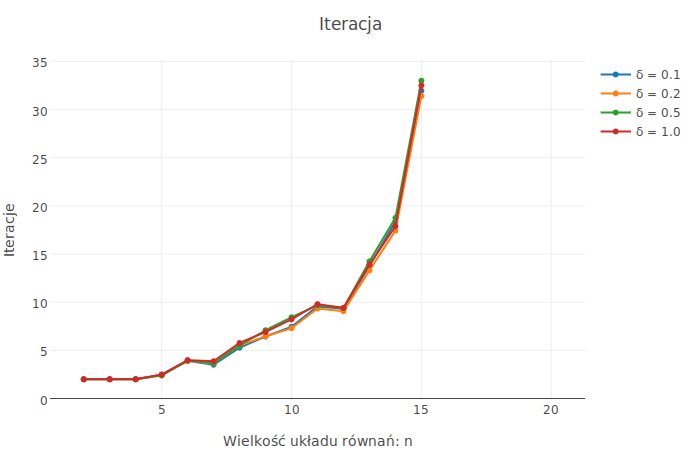
\includegraphics[width=0.9\textwidth]{avg_iterations_V}
    \caption{Średnia ilość iteracji potrzebna do zakończenia metody Newtona dla funkcji V \eqref{eq:V}}
    \label{fig:avgiterationsV}
\end{figure}

\begin{figure}[h]
    \centering
    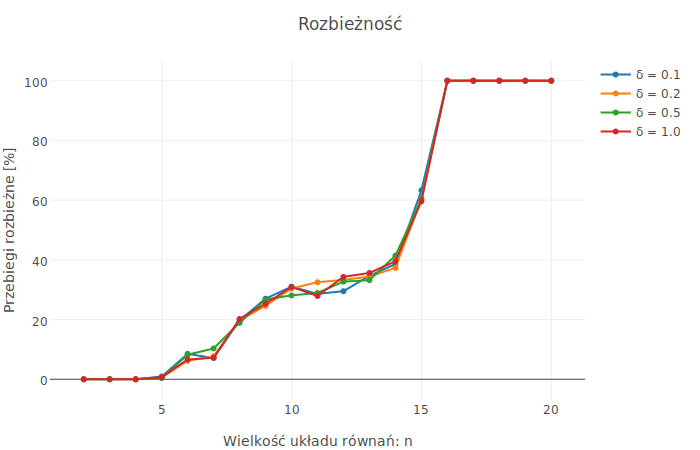
\includegraphics[width=0.9\textwidth]{avg_diversions_V}
    \caption{Procent uruchomień metody Newtona dla funkcji V \eqref{eq:V}, które nie zbiegły w limicie iteracji}
    \label{fig:avgdiversionsV}
\end{figure}

\FloatBarrier
\section{Analiza wyników}

Jak widać na wykresach \ref{fig:relprecision} oraz \ref{fig:norm} metoda Newtona dla funkcji wielu zmiennych nie zawsze jest zbieżna kwadratowo. Tak jak w przypadku funkcji jednej zmiennej, jeżeli pierwiastek którego szukamy jest wielokrotny lub pochodna zeruje się w pierwiastku (funkcje $ F_4 $ i $ F_5 $), to algorytm będzie zbieżny jedynie liniowo.

Dla badanych funkcji generujących duże układy można zaobserwować istotny wpływ przybliżenia początkowego na zbieżność algorytmu, co widać na wykresach \ref{fig:avgdiversionsF} i \ref{fig:avgdiversionsH}. Dla funkcjii $ F $ i $ H $ można także zaobserwować spadek zbieżności metody Newtona wraz z powiększaniem się układu równań (dla parametru $ \delta = 0.5, 1.0 $)

Zbieżność funkcji $ G $ jest natomiast nieczuła zarówno na wielkość układu, jak i przybliżenie początkowe, o ile jest ono względnie blisko $ \bar{x} $, tzn dla $ \delta \leq 0.5 $, co można zaobserwować na wykresie \ref{fig:avgdiversionsG}. Ta funkcja wykazuje także ciekawe zachowanie ilości iteracji względem wielkości układu. Z wykresu \ref{fig:avgiterationsG} widać, że dla $ \delta \leq 0.5 $ metoda Newtona osiąga maksimum potrzebnych iteracji dla $ n = 6 $, po czym ilość ta gwałtownie maleje i stabilizuje się.

Z wykresów \ref{fig:avgiterationsF} oraz \ref{fig:avgiterationsH} (dla $ \delta = 1.0 $ )  można natomiast wywnioskować, że wraz ze wzrostem wielkości układu rośnie ilość iteracji potrzebna do znalezienia miejsc zerowych funkcji $ F $ oraz $ H $. Zarazem widać, że dla $ \delta \leq 0.5 $ obliczenie pierwiastka funkcji H wymaga praktycznie stałej ilości iteracji, niezależnie od wielkości układu.

Przy obliczaniu jakobianu funkcji $ V $ \eqref{eq:V} otrzymamy macierz Vandermonde'a, dla której metoda eliminacji Gaussa od pewnej wielkości macierzy generuje rozwiązania bardzo różne od prawdziwych. Efekt tego zachowania widać na wykresie \ref{fig:avgdiversionsV}, gdzie dla $ n \geq 16 $ metoda Newtona nie jest w stanie znaleźć rozwiązania. 

\section{Wnioski}

Na podstawie wykonanych obliczeń można stwierdzić, że metoda Newtona jest dość pewną metodą rozwiązywania układu równań nieliniowych, o ile potrafimy znaleźć dobre przybliżenie początkowe. Dla większości funkcji jest ona zbieżna kwadratowo. Największym problemem w wykorzystaniu tego algorytmu jest konieczność znania pochodnej funkcji $ F $ która dla dużego układu równań może być trudna do obliczenia. 

\section{Uwagi techniczne}

Aby użyć zaimplementowanej metody Newtona, należy w środowisku interaktywnym zaimportować plik \texttt{program.jl} i wywołać funkcję \texttt{newton(F, J, x)}. Testy najlepiej przeprowadzić za pomocą metody \texttt{show\_set(nr)} gdzie \texttt{nr} jest numerem funkcji dla małych funkcji testowych lub za pomocą metody \texttt{show\_generated(str; size)} gdzie \texttt{str} to jedna z nazw : \emph{polynomial}, \emph{sin\_cos}, \emph{sin\_cos\_2}, \emph{vandermonde}, a size to wielkość układu równań który chcemy wygenerować. Tworzenie wykresów i inne metody pomocnicze są zaprezentowane w zeszycie \texttt{program.ipynb}

\begin{thebibliography}{99}

\bibitem{kincaid} David Kincaid, Ward Cheney, przekł.~Stefan Paszkowski,
\emph{Analiza numeryczna},
Warszawa, WNT, 2006.

\bibitem{ortega} J.~C.~Ortega, W.~C.~Rheinboldt,
\emph{Iterative Solution of Nonlinear Equations in Several Variables},
New York, Academy Press, 1970

\bibitem{bjorck} \r{A}ke Bj\"{o}rck, Germund Dahlquist, przekł.~Stefan Paszkowski
\emph{Metody Numeryczne},
Warszawa, PWN, 1987

\end{thebibliography}

\end{document}